\documentclass{spy}
\course{Time-Domain Astrophysics}
\topic{Variable Stars}

\begin{document}

\tableofcontents

\section{General Comments}
They are found:
\begin{itemize}
    \item across whole range of stellar masses
    \item in many regions of the HRD
    \item in many major phases of stellar evolution
\end{itemize}

They are usually easy to see, as variable.
They provide insights into stellar physics.
They can be used as distance measures, e.g. expansion of Universe, and 3D mapping of SMC, via their period-luminosity relation.


See \url{https://www.aavso.org/}

\section{Classification}
Broad types:
Based on observability:
\begin{itemize}
\item Intrinsic:
    \begin{itemize}
    \item pulsation instability
    \item dynamical instability
    \item explosion
    \end{itemize}
\item Extrinsic, e.g. eclipsing binaries
\end{itemize}

\begin{figure}[ht]
    \centering
    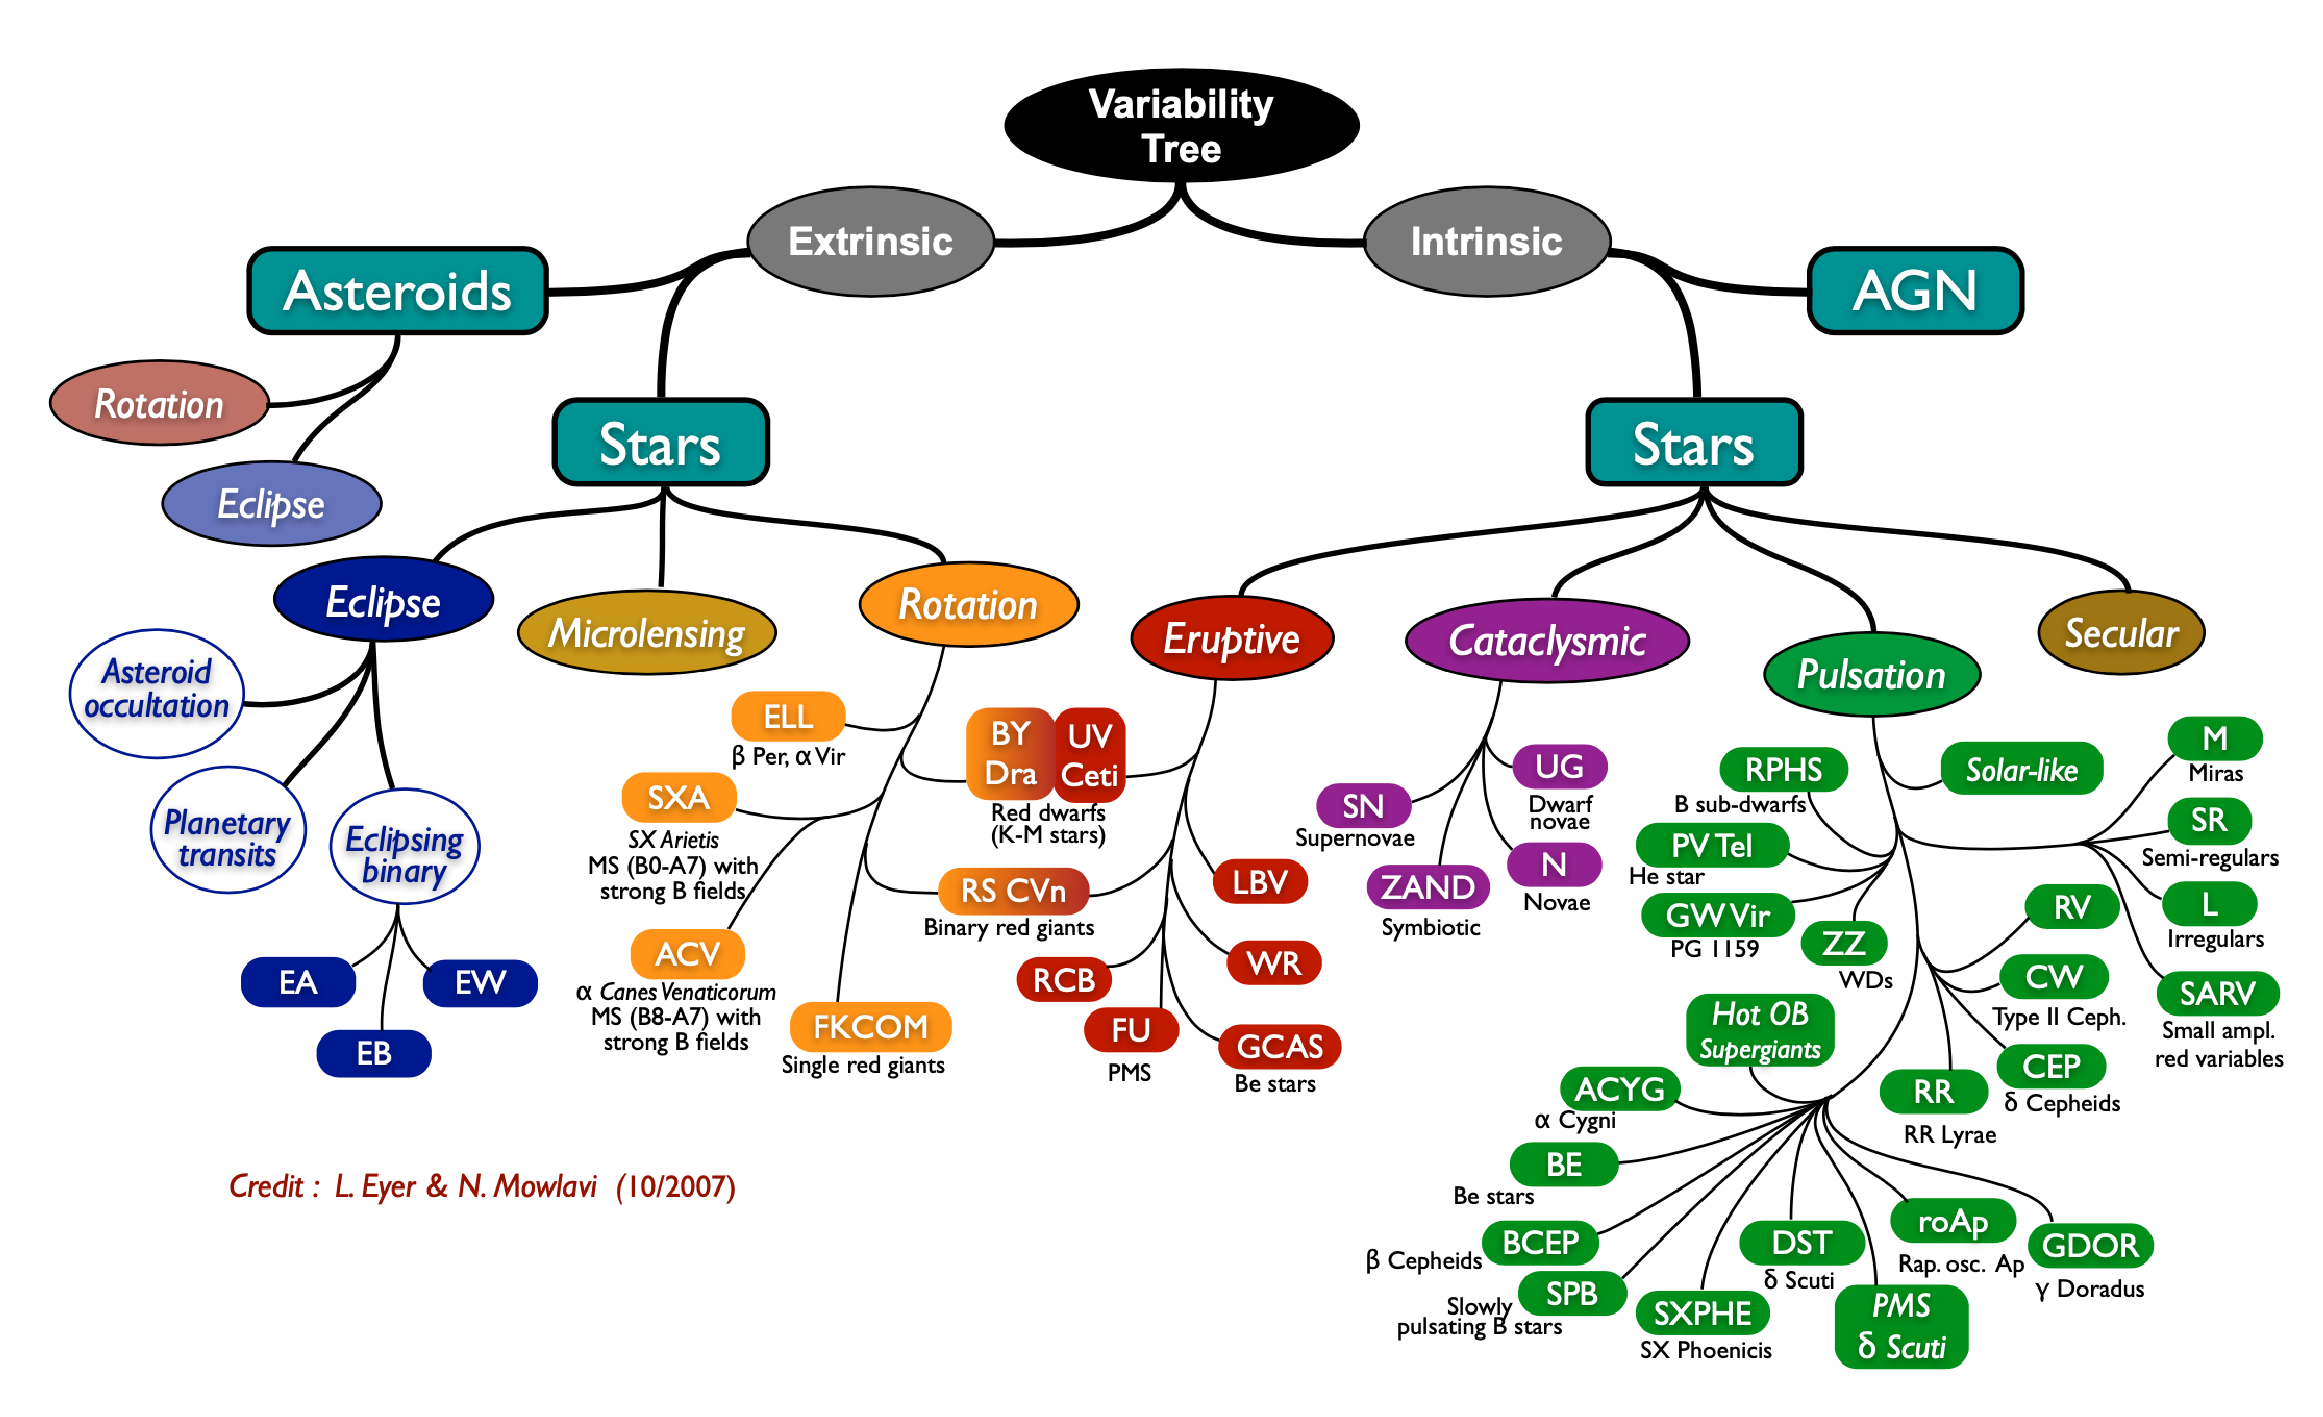
\includegraphics[width=\textwidth]{variable_classes.eps}
    \caption{Classification of Variables. From \citet{eyerVariableStarsObservational2008}}
    \label{variable_classes_diagram}
\end{figure}

Based on observability:
\begin{itemize}
\item Naked-eye (e.g. Mira, Algol, \(\delta\) Cephei)
\item Telescope
\end{itemize}

Based on light-curve features:
\begin{itemize}
\item Period
\item Amplitude (band-dependent)
\item Variability
    \begin{itemize}
    \item Highly regular
    \item Semi-variable
    \item Multi-phase periodic
\end{itemize}\end{itemize}

Based on HRD features:
\begin{itemize}
\item Position on HRD within a group (e.g. WDs, MS, AGB, HB, YSG)
\item Spectral type
\item Luminosity (band-dependent)
\item Colour
\end{itemize}


\section{Physical Factors Influencing Observations}
Factors include:
\begin{itemize}
\item convective zones of star
\item rotation
\item magnetic fields
\item envelope size
\item average density
\item opacity
\item ionisation
\item metallicity/population
\item energy production
\item extinction, reddening or amplification by circumstellar dust
\item stellar wind and mass loss
\item non-eclipsing binarity or trinarty (or multarity)
\end{itemize}

\section{Period-Mean Density Relation}
From Eq. 14.6 Carroll \& Ostlie, period (\(\Pi\)) is given by:
\begin{equation}
    \Pi \approx \sqrt{\frac{3 \pi}{2 \gamma G \overline{\rho}}}
    \propto \overline{\rho}^{-0.5}
\end{equation}

where the 'adiabatic gamma' is:
\begin{equation}
    \gamma \equiv \frac{C_\mathrm{P}}{C_\mathrm{V}}
\end{equation}

Higher AVERAGE density - shorter period. Density signifies evolutionary point of star too. 
e.g. LPVs are giant stars with extended envelopes - low average density, so long period.

WDs compact and dense, hence short period. 


\section{List of Variable Stars and Their Features}
See Fig~\ref{variables_list_table} for a list of characteristics of variables. See Fig~\ref{hrd_variables_diagram} for the position on the HRD.

\begin{figure}[h]
    \centering
    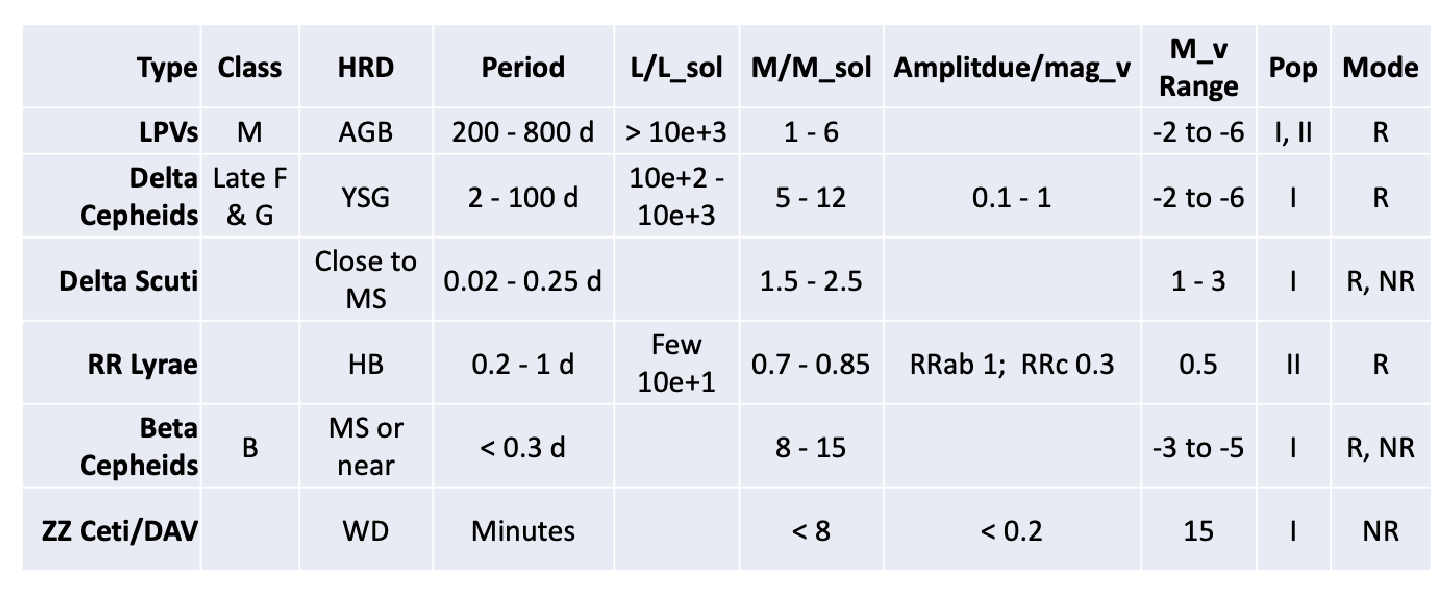
\includegraphics[width=0.9\textwidth]{variables_list.eps}
    \caption{Summary of Characteristics of Variable (Pulsating) Stars}   
    \label{variables_list_table}
\end{figure}

\begin{figure}[ht]
    \centering
    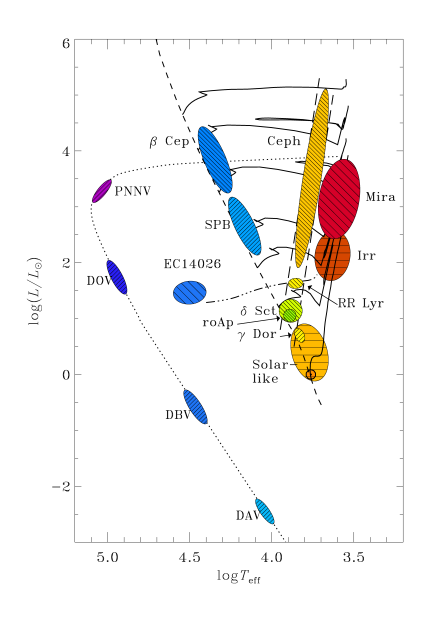
\includegraphics[width=0.8\textwidth]{hrd_variables.eps}
    \caption{Variables on the HRD. From \citet{MiraVariablesPeriod}}
    \label{hrd_variables_diagram}
\end{figure}


\section{Amplitude-Period Relationship}
See Figure~\ref{period_amp_diagram}.

\begin{figure}[ht]
    \centering
    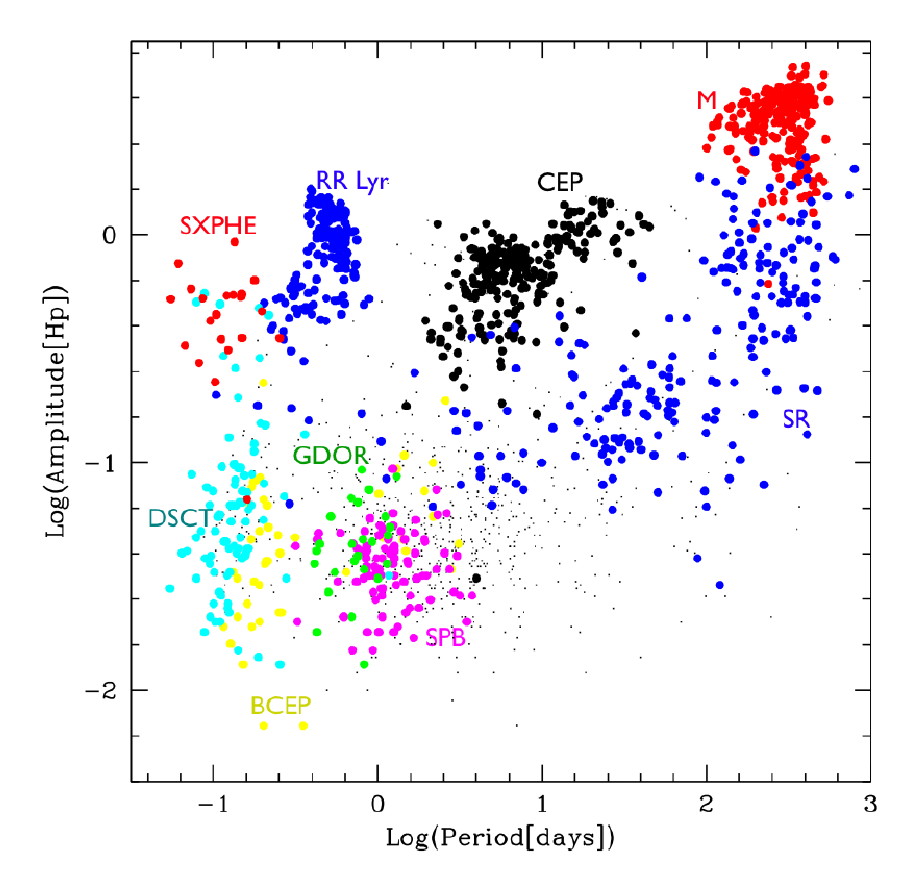
\includegraphics[width=0.8\textwidth]{period_amplitude.eps}
    \caption{Log-Period Log-Amplitude Diagram for Variable Stars. From \citet{eyerVariableStarsObservational2008}}
    \label{period_amp_diagram}
\end{figure}

\section{Radial and Non-Radial Modes, including Spherical Harmonics}
Standing waves cause radial modes, including the fundamental mode, the overtone (harmonic), the second, etc... Organ-pipe analogy. 
\(\delta\) Cepheids and W Virginis stars pulsate in fundamental modes; RR Lyrae in fundamental or first harmonic (or both at same time).  
These sound waves are powered the star as a thermodynamic 'heat engine' (proposed by Eddington). 

There are driving forces and damping forces. When damping forces prevail, no pulsation is seen. When driving forces exceed damping forces, pulsation starts. An equilibrium is reached when driving forces cannot exceed damping forces any more. 

Non-radial pulsations follow spherical harmonics, described by the following mathematics:
\begin{equation}
    Y^l_m (\theta, \phi) = 
\end{equation}

\section{Thermodynamics}
Work done as the gases pulsate is \(P \,dV\). 
Net positive work for the cycle drives oscillations, i.e.
\begin{equation}
    \oint P \,dV > 0
\end{equation}
A cycle will do work if it receives heat when it is in its compressed portion of the cycle, and gives off heat when it is in its expanded portion.
A Carnot cycle, showing hysteresis in P-V parameter space.

What mechanisms can add heat in this compressed phase, and then only in narrow strips on the HRD?

\subsection{The Nuclear '\(\epsilon\) Mechanism'}
\begin{equation}
\epsilon \propto T^\nu
\end{equation}
Compression at centre of star increases energy generation (due to increased temperature and density). However may not contribute to pulsation as the pulsation amplitude of the node at the centre is small. Also, don't see many pulsating stars on the MS of the HRD.

\subsection{The '\(\kappa\) Mechanism' ("Eddington's Valve)}
Usualy Kramer's Law (due to bound electrons in metals) is obeyed:
\begin{equation}
    \kappa \propto \rho T^{-3.5}
\end{equation}
where compression increases temperature far more than density, and radiative opacity decreases, because electrons are stripped from metals. 

Under special circumstances, this relationship changes. (\(\kappa\)) can increase with temperature due to partial ionisation (e.g. He\(^+\) [He II] to He\(^{++}\) [He III] in RR Lyrae and Cepheids), trapping EM radiation/heat, favouring pulsation.  

With the abundance of H and He, during partial re-ionisation of H and He a heat sink occurs where temperature remains fairly constant. This allows recombination of metals and electrons as density increases (but not temperature), increasing opacity. 

H and He II partial ionisation zones exist, at \(1 \times 10^4\)K and \(4 \times 10^4\) K respectively. In stars hotter than F-class, the ionisation zones coincide with convective zones, so NO radiative opacity. In cooler stars, the partial ionisation zones are too deep to make much impact at the surface. Hence the narrow instability strip where RR Lyra.

See Figure~\ref{ionisation_temp_diagram} for a diagram of partial reionisation areas in a star as a function of effective temperature. 

\begin{figure}[h]
    \centering
    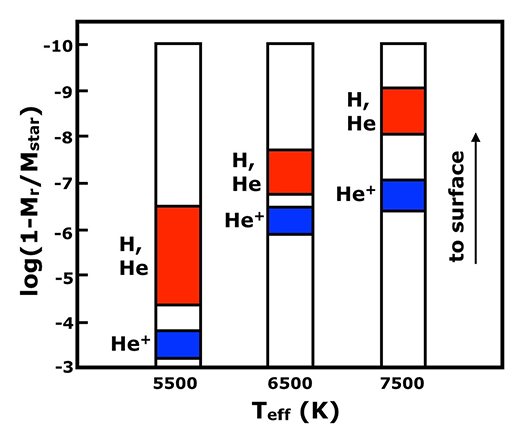
\includegraphics[width=0.4\textwidth]{ionisation_temp.eps}
    \caption{Partial Re-ionisation Depths Depending on Stellar Effective Temperature} 
    \label{ionisation_temp_diagram}
\end{figure}

In the pulsating B stars (e.g. \(beta\) Cepheids), there is an 'iron opacity bump' mechanism - Fe increases opacity at \(1-2 \times 10^5\) K. 

\subsection{The '\(\gamma\) Mechanism'}
Amplifies the \(kappa\)-mechanism. Akin to a phase transition (like ice to liquid water). Energy goes in, but temperature doesn't go up (as much as would be expected). Part of the work done causes further ionisation (increasing specific heats - Cv and Cp), rather than increasing temp.

\section{One-Zone Model}
The one-zone (Zhevakin's) model is shown in Figure~\ref{one_zone_model_diagram}

\begin{figure}[h]
    \centering
    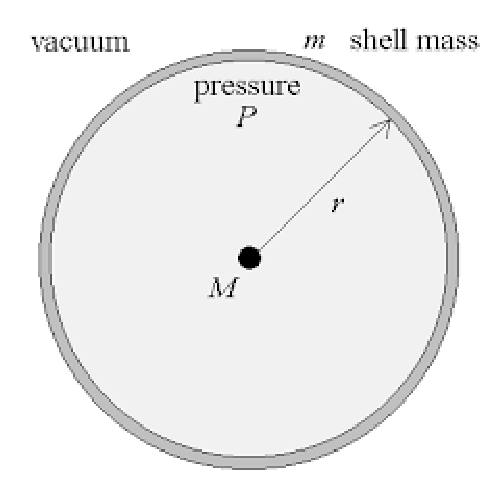
\includegraphics[width=0.2\textwidth]{one_zone_model.eps}
    \caption{The One-Zone Model} 
    \label{one_zone_model_diagram}
\end{figure}

N2L equation of \textit{radial} motion:
\begin{equation}
    \rho \frac{d^2r}{dt^2} = -G \frac{M_r \rho}{r^2} - \frac{dP}{dr}
\end{equation}



\section{The Finite Fourier Transform}
\begin{equation}
F_\mathrm{T}(\nu) = \int_{-T/2}^{T/2} f(t)e^{-i 2\pi \nu t} \,dt
\end{equation}

\section{Period-Luminosity (P-L) Relation - the Leavitt Law}

Published by Henrietta Leavitt in 1912 \citep{leavittPeriods25Variable1912}. Figure~\ref{leavitt_period_luminosity_diagram} shows the original figure from the 1912 paper, with log period vs apparent magnitude for the 25 SMC Cepheids.

\begin{figure}[ht]
    \centering
    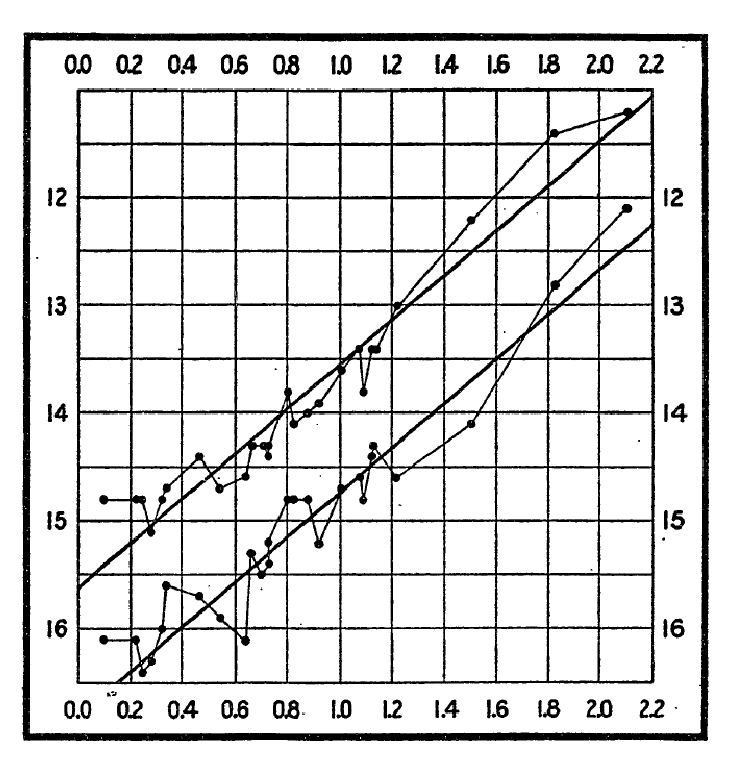
\includegraphics[width=0.6\textwidth]{leavitt_period_luminosity.eps}
    \caption{Log-Period vs Apparent Magnitudes (and their amplitude of change) for 25 Cepheids in the SMC. From \citet{leavittPeriods25Variable1912}}    \label{leavitt_period_luminosity_diagram}
\end{figure}

\subsection{Period-Luminosity-Colour (PLC) Relation}

\subsection{Calibration of the Cepheid PL Relation}
Methods
\begin{itemize}
    \item Parallax
        \begin{itemize}
        \item Direct parallax (Hipparcos satellite)
        \item Gaia
        \end{itemize}
    \item Open cluster main-sequence fitting
    \item Baade-Wesselink method
\end{itemize}

\citet{fouqueNewCalibrationGalactic2007} compared V-band and K-band measurements - K-band was brighter and tighter (Figure~\ref{fouque_cepheid})

\begin{figure}[ht]
    \centering
    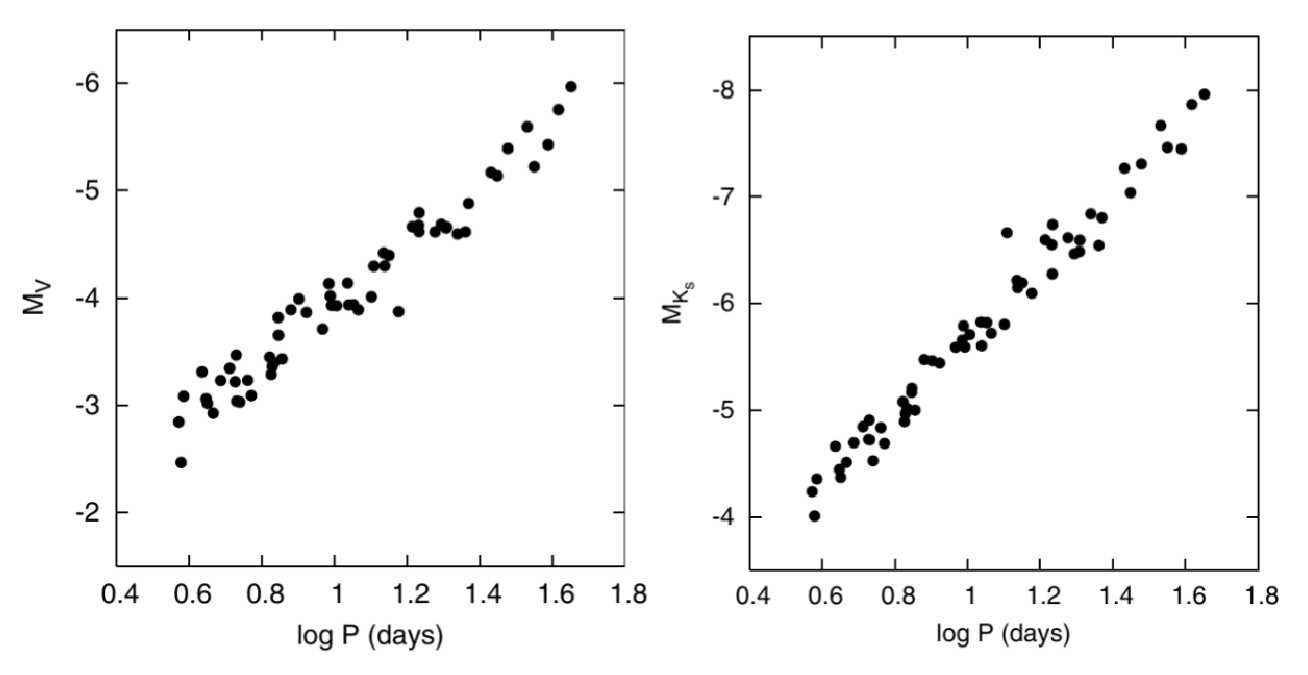
\includegraphics[width=0.7\textwidth]{fouque_cepheid.eps}
    \caption{V-Band vs K-Band calibration of the PL relation for Cepheids in the the Milky Way and LMC. From \citet{fouqueNewCalibrationGalactic2007}}   
    \label{fouque_cepheid}
\end{figure}

The distance modulus:
\begin{equation}
\mu \equiv m-M = 5\log_\mathrm{10}(d) - 5
\end{equation}

Cepheids, primary distance indicators, are exceedingly bright YSGs. Ground-based telescopes can see them a few Mpc away; HST up to 20 Mpc. 

LPVs are a complex zoo of variables - PL relations are varied. 

\section{Baade-Wesselink(-Becker) Method}

Start with:
\begin{equation}
    L = 4 \pi R^2 \sigma T_\mathrm{eff}
\end{equation}
Take logs and multiply by -2.5:
\begin{equation}
    M = a \log_\mathrm{10}(R) + b \log_\mathrm{10}(T_\mathrm{eff})
\end{equation}
Subtract end phase from start phase of pulsation:
\begin{equation}
    M_\mathrm{1}- M_\mathrm{2}= a \log_\mathrm{10}(R_\mathrm{1}/R_\mathrm{2}) + b \log_\mathrm{10}(T_\mathrm{eff,1}/T_\mathrm{eff,2})
\end{equation}
Difference in apparent mags same as difference in absolute mags, so:
\begin{equation}
    \Delta m \equiv m_\mathrm{1}- m_\mathrm{2}= a \log_\mathrm{10}(R_\mathrm{1}/R_\mathrm{2}) + b \log_\mathrm{10}(T_\mathrm{eff,1}/T_\mathrm{eff,2})
\label{baade_1}
\end{equation}
Measure \(m_\mathrm{1}\), \(m_\mathrm{2}\), and \(T_\mathrm{eff}\), then measure radial velocity (\(V_\mathrm{R}\)), the change in radius w.r.t. time:
\begin{equation}
    V_\mathrm{R}(t) = \frac{dR}{dt}
\end{equation}
Therefore:
\begin{equation}
    R = \int V_\mathrm{R}(t) \,dt
\end{equation}
Thus:
\begin{equation}
    R_\mathrm{2} - R_\mathrm{1} = \int_{t_\mathrm{1}}^{t_\mathrm{2}} V_\mathrm{R}(t) \,dt
\label{baade_2}
\end{equation}
Combine Eq.(\ref{baade_1}) and Eq.(\ref{baade_2}) to give 2 equations with 2 unknowns, and can then solve for \(R_\mathrm{1}\) and \(R_\mathrm{2}\).
Repeat multiple times over whole pulsation cycle, to get average radius.
Nowadays interferometry can be used to measure radius. 


\bibliographystyle{mnras}
\bibliography{variables_bibliography}

\end{document}
